\section{Aufbau und Durchführung}
\label{sec:durchfuehrung}
Die spezifische Wärmekapazität soll unter konstantem Druck bestimmt werden, da dabei weniger messtechnische Probleme auftreteten, als bei der Messung unter konstantem Volumen.
Für die Messung wird ein Mischungskalorimeter, welches in Abbildung \ref{fig:aufbau} dargestellt ist, verwendet. Allerdings werden die Proben nicht mit Heizbaken sondern in einem Wasserbad erhitzt. Zum Bestimmen der Massen der Proben dient eine Schnellwage.
Für die Messung der Temperaturen wird ein Thermoelement verwendet, da es sich schneller auf die Temperatur einstellt als ein digitales Thermometer. Dieses besteht aus zwei Metallen, welche unterschiedliche Austrittsarbeiten der Elektronen besitzen. Die beiden Metalle sind an einer Stelle verbunden. An dieser Stelle gehen Elektronen von dem Metall mit der kleineren Austrittsarbeit in das mit Größerer über, bis das dadurch auftretende Potential dem entgegenwirkt. Diese Spanung wird als Kontaktpotential bezeichnet. Wird nun ein Metall erwärmt, gleichen sich die Kontaktpotentiale nicht mehr aus und die sogenannte Thermospannung $U_\mathrm{th}$ ist messbar.
Aus dieser lässt sich mit
\begin{equation}
  T = 25,157 U_\mathrm{th} - 0,19 U_\mathrm{th}^2
\end{equation}
die Temperatur berechnen. Die Thermospannung ist hier in \si{\milli\volt} gegeben. Da es sich bei der so berechneten Temperatur um die Temperaturdifferenz der beiden Kontaktstellen handelt, befindet sich ein Kontakt in Eiswasser mit $T=0$. Somit ist die berechnete Temperaturdifferenz direkt die gesuchte Temperatur.

\begin{figure}
  \centering
  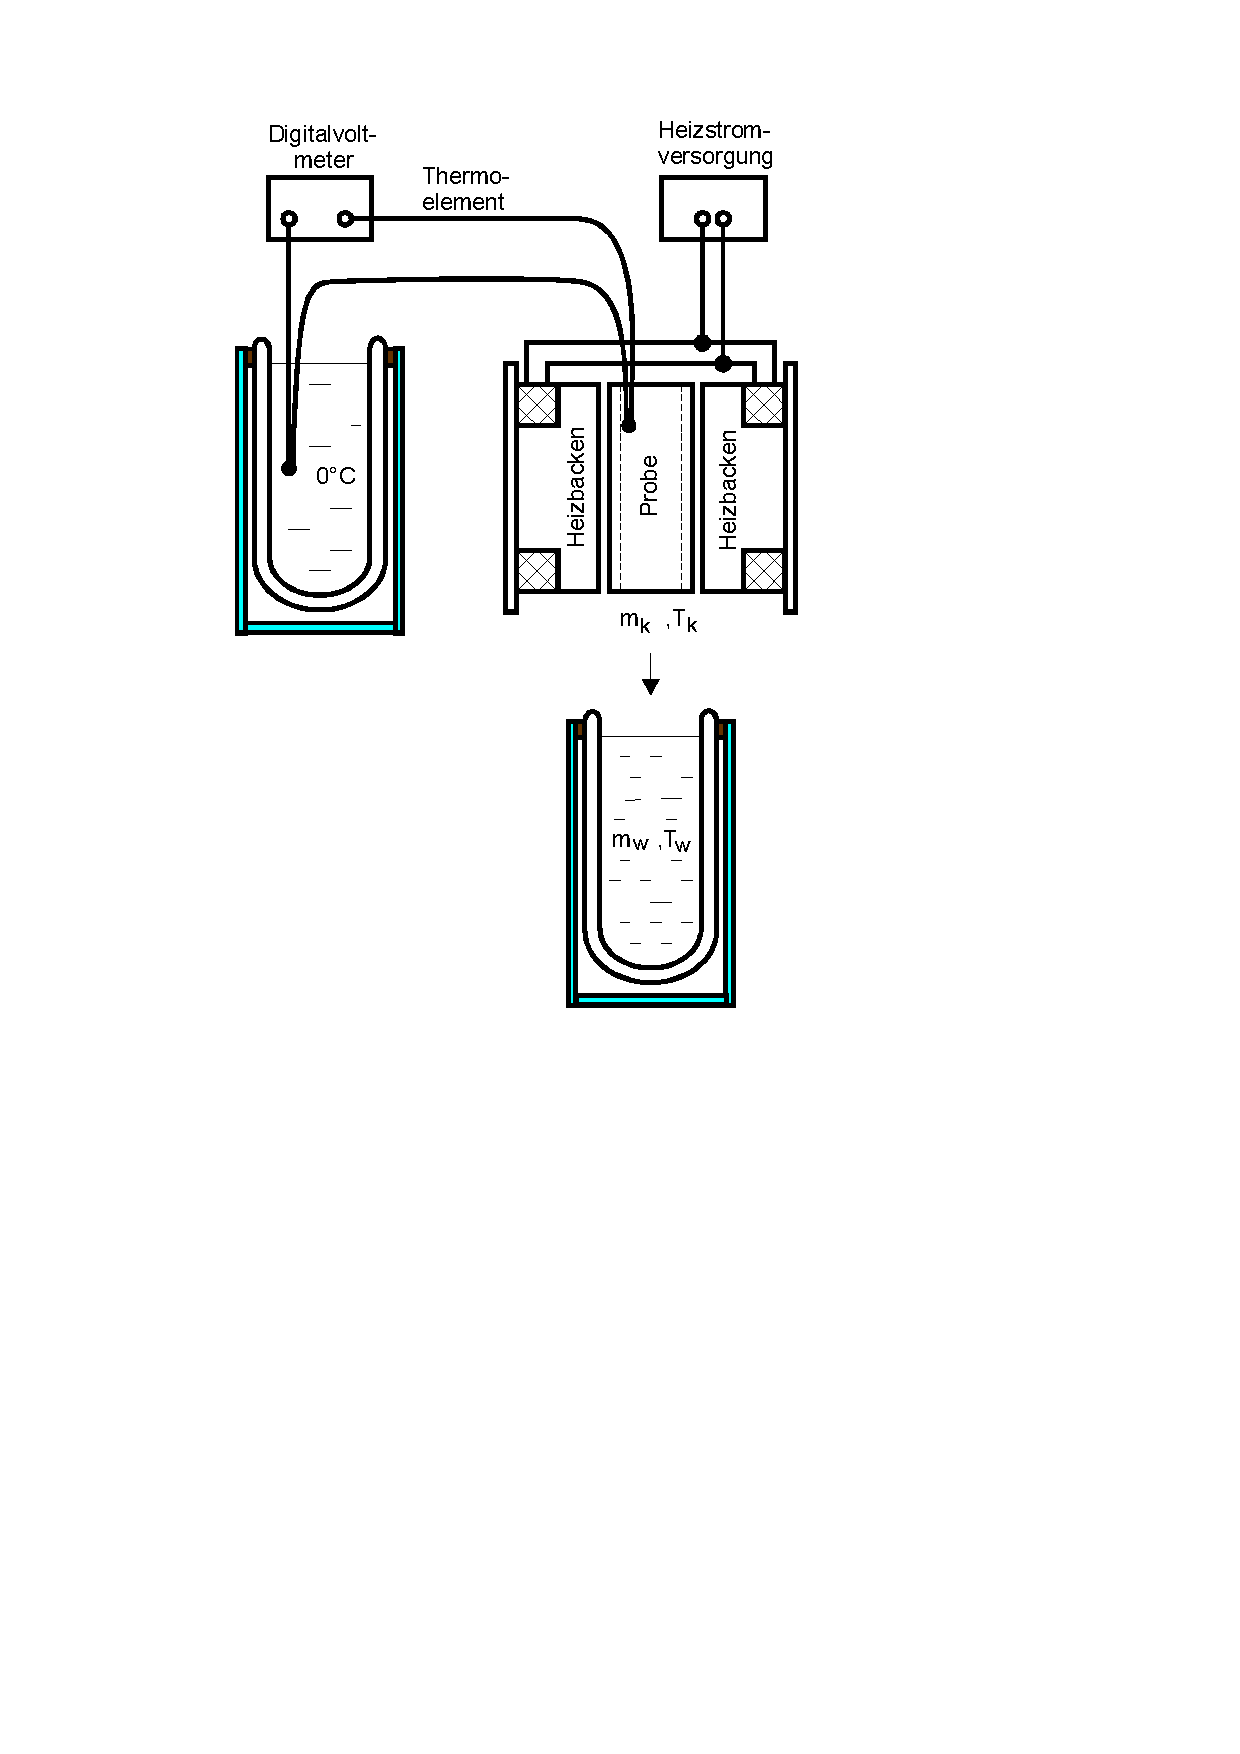
\includegraphics[scale=0.6]{content/aufbau.pdf}
\caption{Schematische Darstellung der Messapparatur \cite{anleitung201}.}
  \label{fig:aufbau}
\end{figure}

\subsection{Bestimmung der Wärmekapazität des Mischungskalorimeters}
 Um die Wärmekapazität des Kalorimeters zu bestimmen, werden zwei Wassermengen mit verschiedenen Temperaturen vermischt.   Die Wärmekapazität des Mischungskalorimeters ergibt nach \ref{eqn:cgmg}. Somit müssen sowohl die Masse als auch die Temperatur der beiden Wassermengen bekannt sein. Die Masse des Wassers wird mit einer Schnellwage bestimmt und die Temperatur beziehungsweise die Thermospannung wird gemessen. Die Hälfte des Wassers wird in ein anderes Gefäß gefüllt und erhitzt. Bevor es zu dem noch kalten Wasser im Mischungskalorimeter gegeben wird, wird die Thermospannung gemessen. Sobald die Temperatur konstant ist, wird diese als Mischungstemperatur $T_\mathrm{m}$ aufgenommen.

\subsection{Bestimmung der Wärmekapazitäten der Stoffe}
Zunächst werden die Massen $m_\mathrm{k}$ der Proben mit Hilfe einer Schnellwage bestimmt. Ebenso wird die Masse des sich im Mischungskalorimeter $m_\mathrm{W}$ befindenden Wassers mittels Schnellwage ermittelt.
Der Probenkörper wird in einem Wasserbad erhitzt und die dann erreichte Temperatur $T_\mathrm{K}$ gemessen. Auch die Temperatur des Wasser $T_\mathrm{W}$ im Mischungskalorimeter wird vor dem Eintauchen des Probenkörpers gemessen. Findet kein Wärmeaustausch mehr zwischen Probe und Wasser statt, wird die Mischungstemperatur $T_\mathrm{m}$ aufgenommen.
Für Zinn wird der beschriebene Vorgang drei mal wiederholt.
